% Autor: Daniel Tatzel

\section{Gästebuch}

\subsection{Gästebuch ausgeloggt}

Jeder Benutzer hat die Möglichkeit das Gästebuch der Die Tutoren AG einzusehen. \newline Um ins Gästebuch schreiben zu können ist es nötig, angemeldet zu sein.
\begin{figure}[!htbp]
\centering
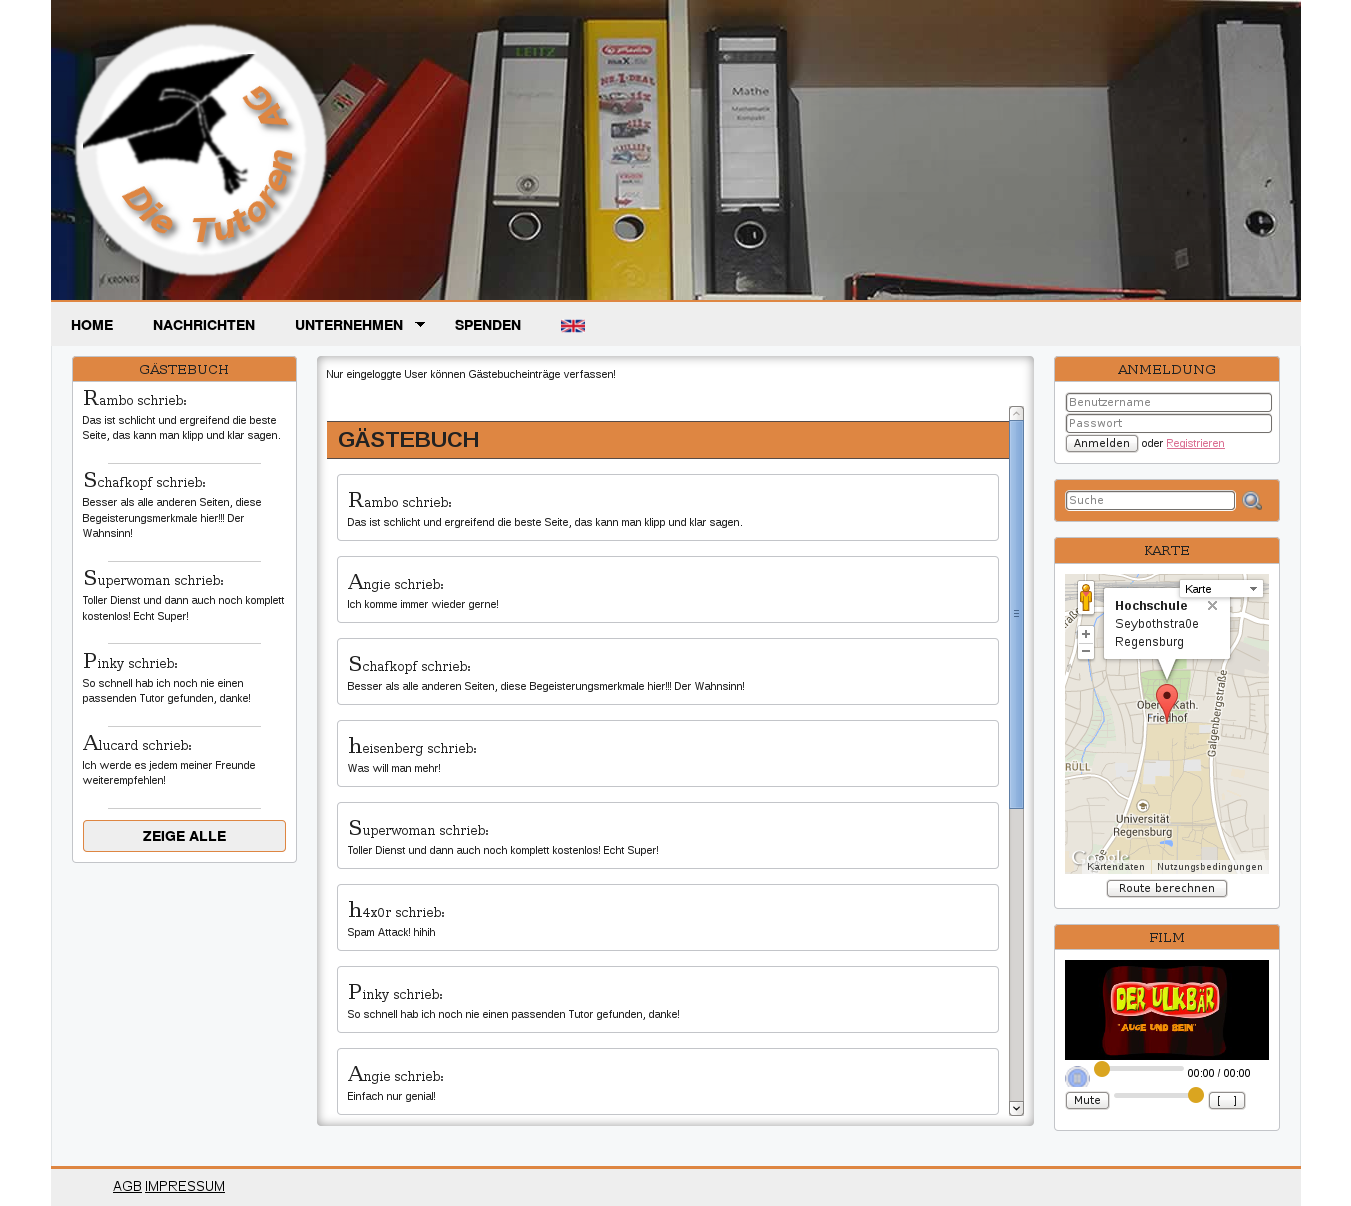
\includegraphics[width=1\linewidth]{../Screenshots/de/Gaestebuch}
\caption{Gästebuch ausgeloggt}
\label{fig:Gaestebuch}
\end{figure}

\newpage
\subsection{Gästebuch eingeloggt}

Eingeloggte Benutzer können über das Formular neue Gästebucheinträge hinzufügen.

\begin{figure}[!htbp]
\centering
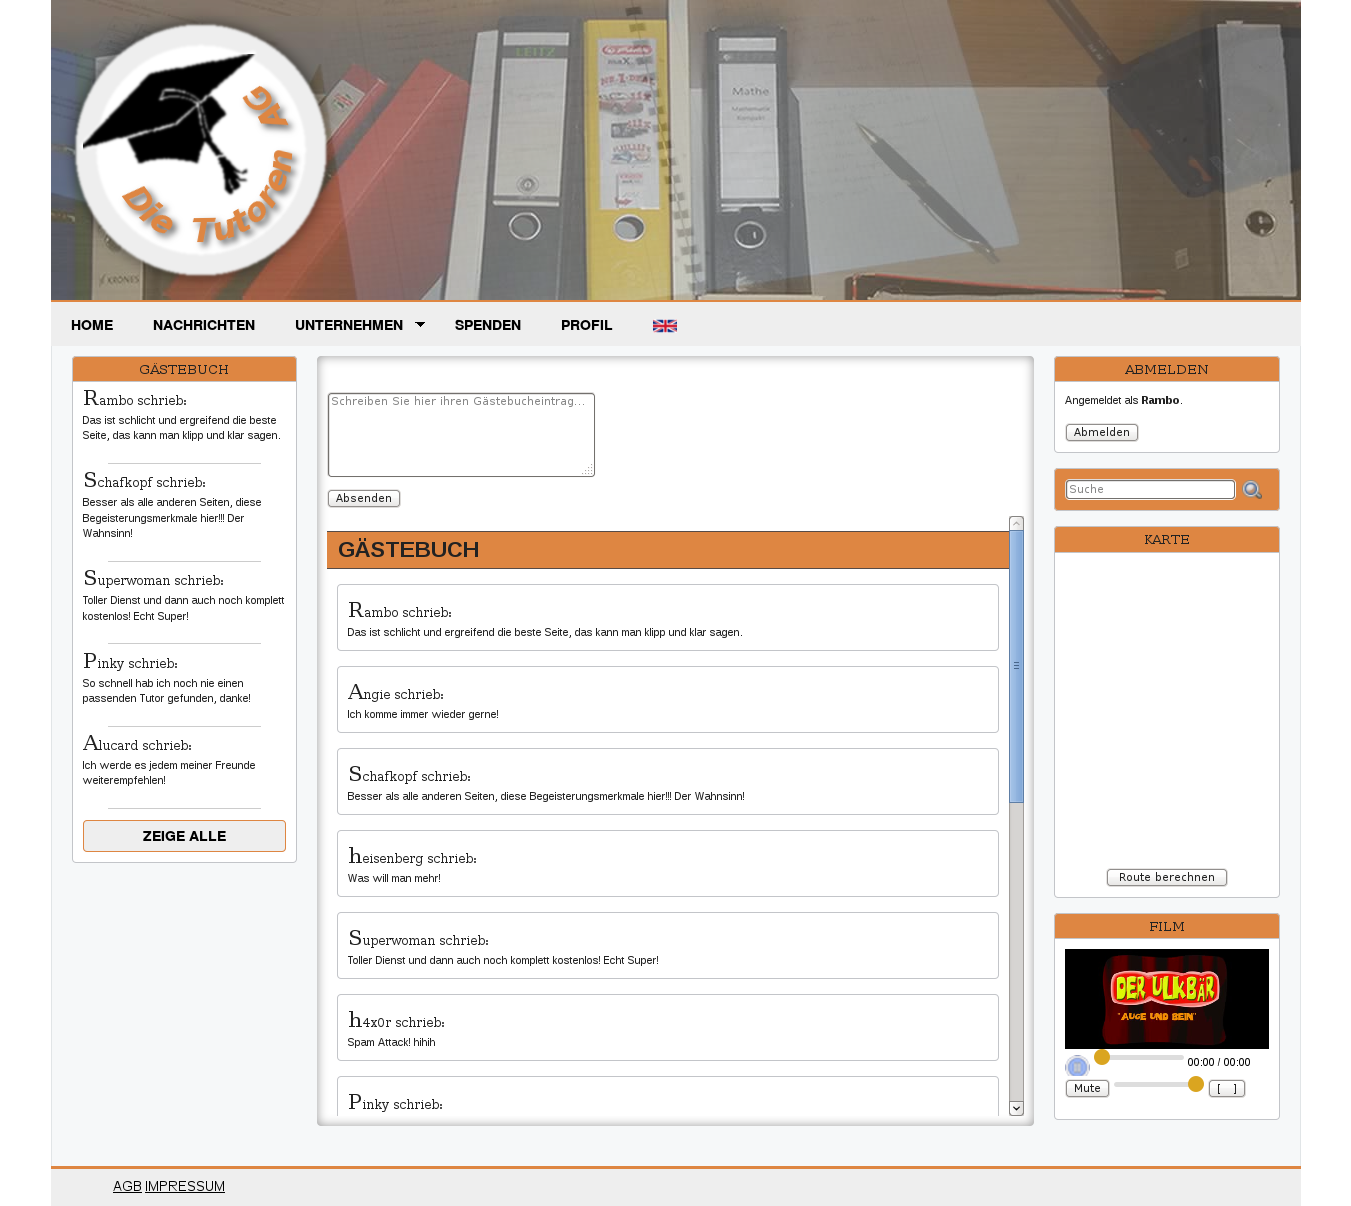
\includegraphics[width=1\linewidth]{C:/Users/Frostbite/Documents/YWEE/Meins2/Documents/Doku/Screenshots/de/Gaestebuch_logged_in}
\caption{Gästebuch eingeloggt}
\label{fig:Gaestebuch_logged_in}
\end{figure}


\newpage

\subsection{Top-Gästebuch}

Auf der Startseite kann jeder Benutzer die Besten abgegebenen Gästebuchkommentare betrachten und wird auf Wunsch zum kompletten Gästebuch weitergeleitet (siehe Pfeil).

\begin{figure}[!htbp]
\centering
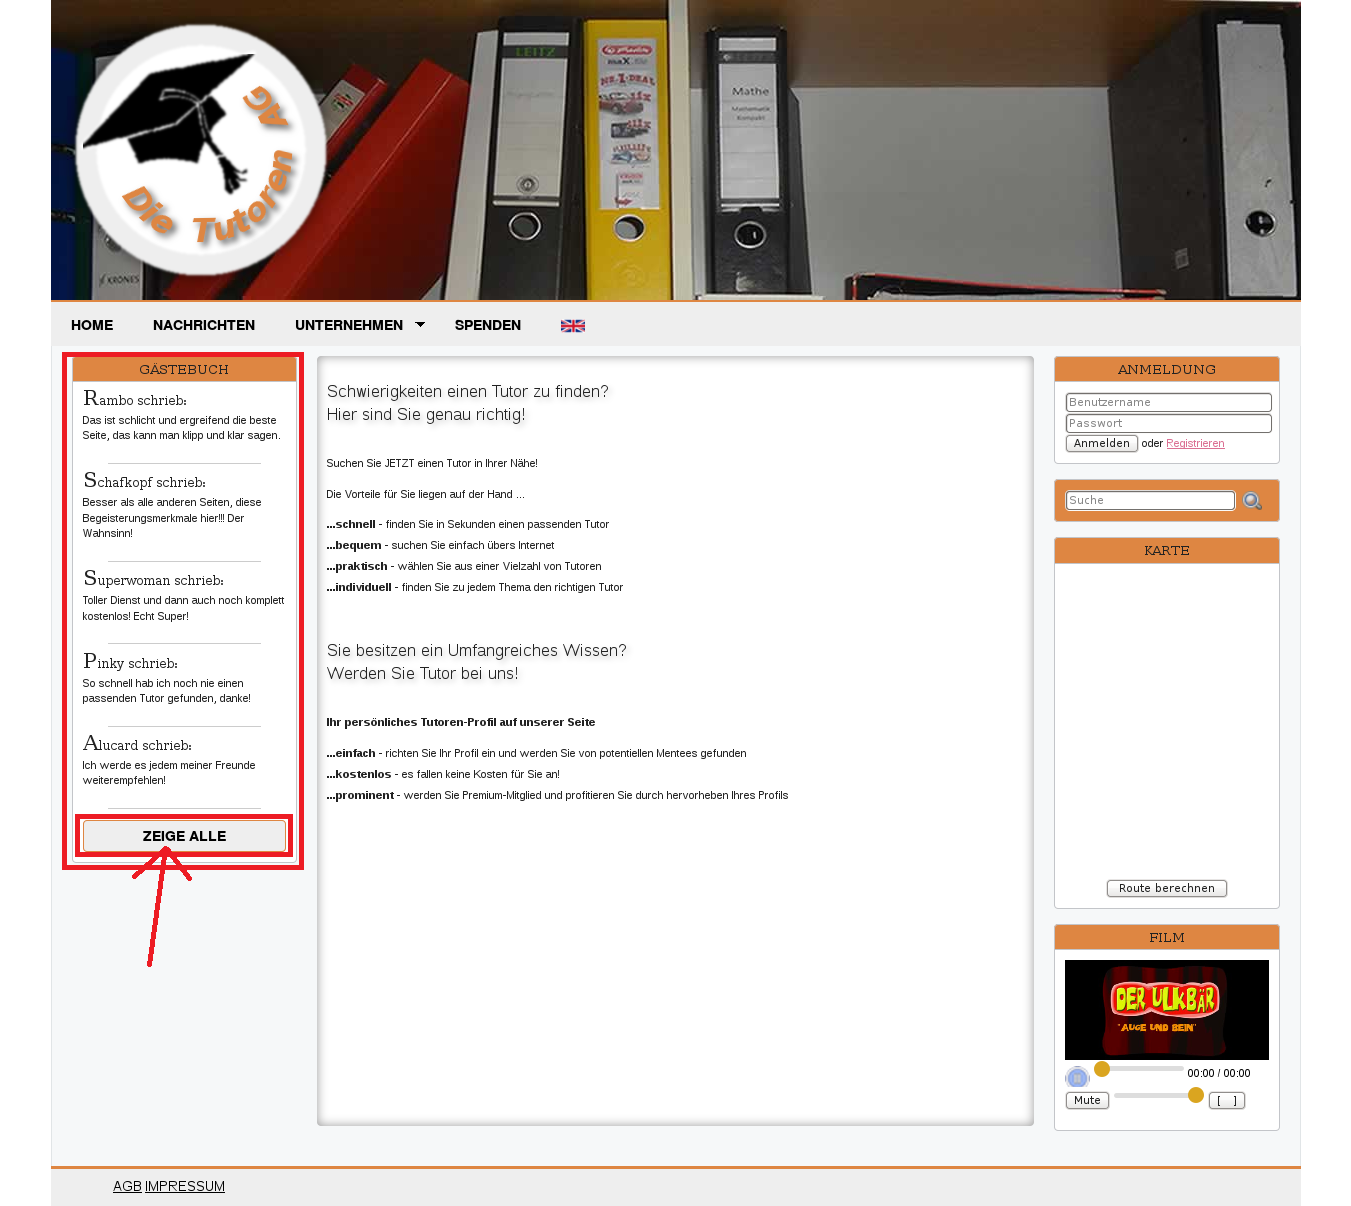
\includegraphics[width=1\linewidth]{C:/Users/Frostbite/Documents/YWEE/Meins2/Documents/Doku/Screenshots/de/TopGaestebuch}
\caption{Top Gästebucheinträge}
\label{fig:TopGaestebuch}
\end{figure}
